% DRAFT Figure 1: the I2SB chain from the current T1 to the synthesized CT1, with the conditioning
% injected into the network at every step. Tiles: one test case (slice 81); intermediates are the
% bridge's closed-form marginal between the two ends under the trained schedule (illustrative).
\documentclass[border=6pt]{standalone}
\usepackage{tikz}
\usetikzlibrary{arrows.meta,positioning,calc,fit,backgrounds}
\usepackage[T1]{fontenc}
\usepackage{lmodern}

\definecolor{net}{HTML}{2A78D6}
\definecolor{cond}{HTML}{EB6834}
\definecolor{ink}{HTML}{0B0B0B}
\definecolor{muted}{HTML}{52514E}

\newcommand{\tile}[3]{% name, node name, width
  \node[inner sep=0pt, draw=muted, line width=0.3pt] (#2) {\includegraphics[width=#3]{#1}};}

\begin{document}
\begin{tikzpicture}[font=\small, >={Stealth[length=2.2mm]},
  netbox/.style={draw=net, fill=net!8, rounded corners=2pt, line width=0.7pt,
                 minimum width=1.25cm, minimum height=0.95cm, align=center, font=\footnotesize},
  flow/.style={->, line width=0.8pt, ink},
  inj/.style={->, line width=0.8pt, cond}]

  \def\tw{2.3cm}
  % ---- the chain ------------------------------------------------------------------------
  \node[inner sep=0pt, draw=muted, line width=0.3pt] (x1)  at (0,0)    {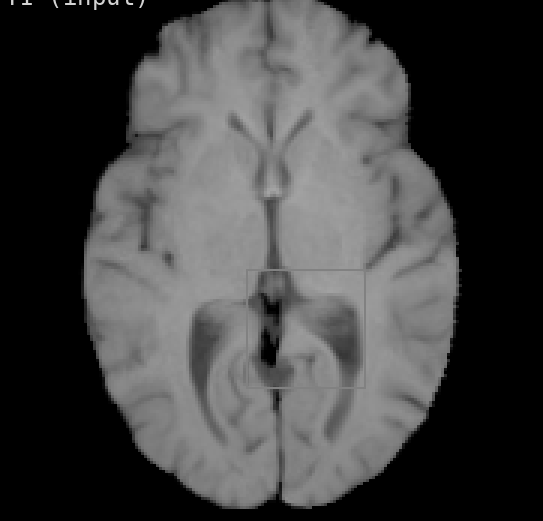
\includegraphics[width=\tw]{t1.png}};
  \node[inner sep=0pt, draw=muted, line width=0.3pt] (x75) at (4.3,0)  {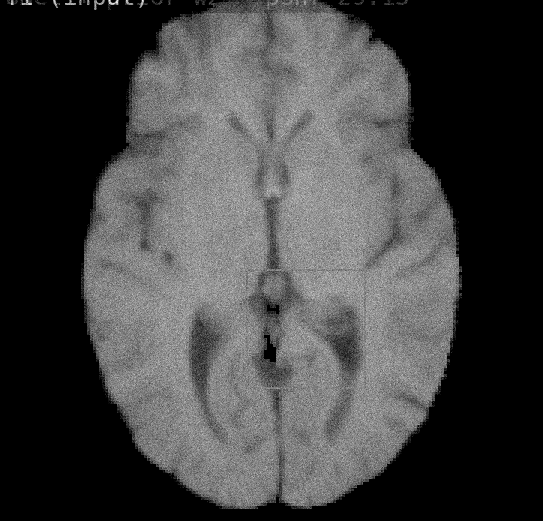
\includegraphics[width=\tw]{xt_75.png}};
  \node[inner sep=0pt, draw=muted, line width=0.3pt] (x50) at (8.6,0)  {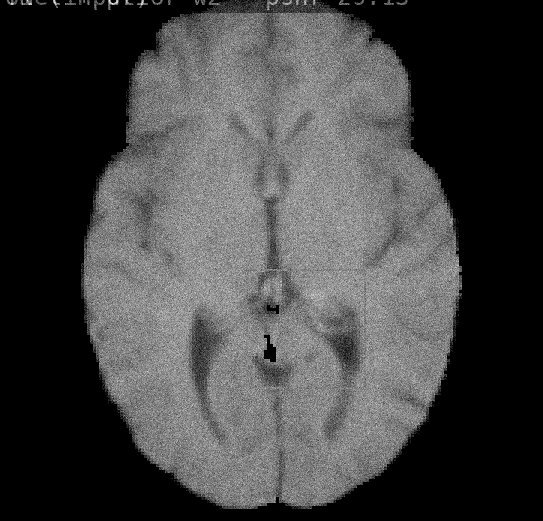
\includegraphics[width=\tw]{xt_50.png}};
  \node[inner sep=0pt, draw=muted, line width=0.3pt] (x25) at (12.9,0) {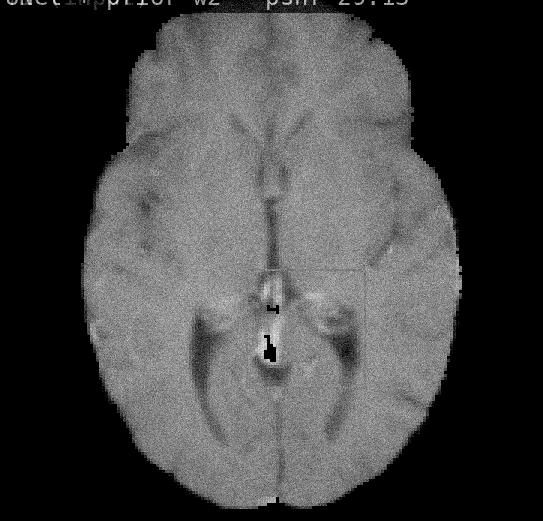
\includegraphics[width=\tw]{xt_25.png}};
  \node[inner sep=0pt, draw=muted, line width=0.3pt] (x0)  at (17.2,0) {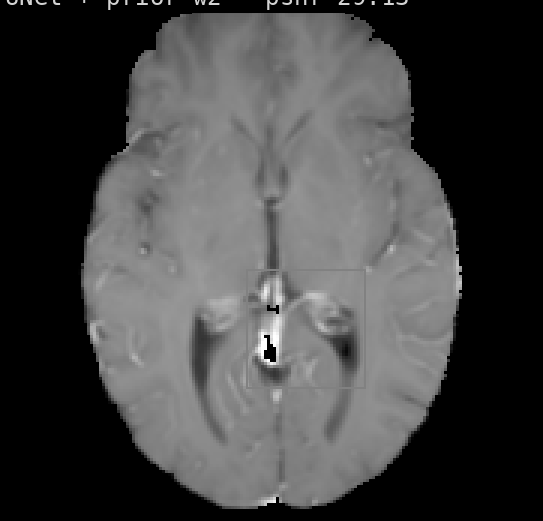
\includegraphics[width=\tw]{longi.png}};

  \foreach \a/\b/\n in {x1/x75/n1, x75/x50/n2, x50/x25/n3, x25/x0/n4} {
    \node[netbox] (\n) at ($(\a.east)!0.5!(\b.west)$) {U-Net\\[-1pt]$\hat x_0(x_t)$};
    \draw[flow] (\a.east) -- (\n.west);
    \draw[flow] (\n.east) -- (\b.west);
  }

  % labels under the tiles
  \node[below=2pt of x1, align=center]  {$x_1$: current T1\\(measured, $t{=}1$)};
  \node[below=2pt of x75, align=center] {$x_{t}$, $t{=}0.75$};
  \node[below=2pt of x50, align=center] {$x_{t}$, $t{=}0.5$};
  \node[below=2pt of x25, align=center] {$x_{t}$, $t{=}0.25$};
  \node[below=2pt of x0, align=center]  {$\hat x_0$: synthesized CT1\\($t{=}0$)};

  % time axis
  \draw[->, muted, line width=0.6pt] ($(x1.south west)+(0,-1.25)$) -- ($(x0.south east)+(0,-1.25)$)
    node[pos=0, anchor=north west, font=\footnotesize, muted] {$t=1$: start at the patient's own anatomy}
    node[pos=1, anchor=north east, font=\footnotesize, muted] {$t=0$};
  \node[font=\footnotesize, muted] at ($(x50.south)+(0,-2.0)$)
    {20 steps; each: U-Net predicts $\hat x_0$, the bridge posterior gives the next $x_t$};

  % ---- the conditioning, injected at every step -------------------------------------------
  \coordinate (bus) at ($(x1.north)+(0,1.2)$);
  \draw[cond, line width=1.1pt] ($(n1.north)+(-0.0,1.53)$) -- ($(n4.north)+(0,1.53)$);
  \foreach \n in {n1,n2,n3,n4}
    \draw[inj] ($(\n.north)+(0,1.53)$) -- (\n.north);
  \node[cond, font=\footnotesize, anchor=south] at ($(n2.north)!0.5!(n3.north)+(0,1.55)$)
    {same conditioning, input channels of the U-Net at every step};

  % current exam (left) and registered prior (right), feeding the bus
  \begin{scope}[shift={($(x1.north)+(-0.1,3.6)$)}]
    \foreach \i in {2,1,0}
      \node[inner sep=0pt, draw=muted, line width=0.3pt, fill=white] (c\i) at (0.18*\i,0.18*\i)
        {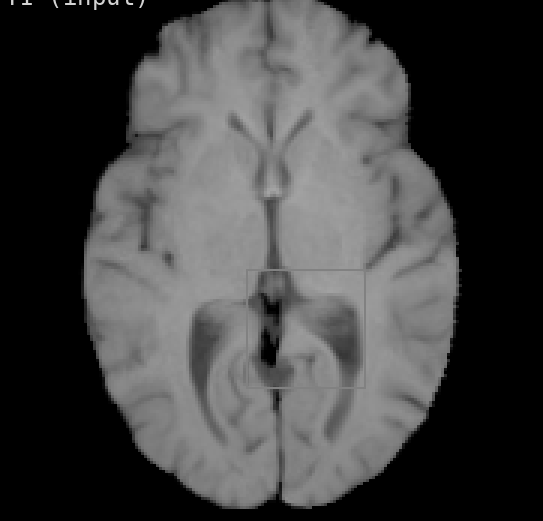
\includegraphics[width=1.35cm]{t1.png}};
    \node[align=center, font=\footnotesize, anchor=north] at (0.18,-0.8)
      {current FLAIR, T1, T2\\[-1pt]\textcolor{red}{(draft: T1 tile ×3)}};
  \end{scope}
  \begin{scope}[shift={($(x0.north)+(-0.6,3.6)$)}]
    \foreach \i in {4,3,2,1,0}
      \node[inner sep=0pt, draw=muted, line width=0.3pt, fill=white] (p\i) at (0.16*\i,0.16*\i)
        {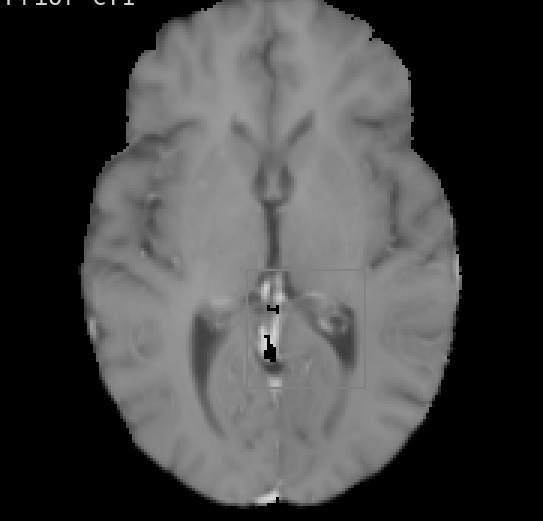
\includegraphics[width=1.35cm]{prior_ct1.png}};
    \node[align=center, font=\footnotesize, anchor=north] at (0.3,-0.8)
      {prior T1 \& CT1, slices $z{-}2\ldots z{+}2$\\[-1pt]registered with FLAIR/T1/T2 only};
  \end{scope}
  \draw[cond, line width=1.1pt] ($(c0.south)+(0,-1.3)$) |- ($(n1.north)+(0,1.53)$);
  \draw[cond, line width=1.1pt] ($(p0.south)+(0.3,-1.3)$) |- ($(n4.north)+(0,1.53)$);
\end{tikzpicture}
\end{document}
